\documentclass{ximera}
\input{../preamble.tex}

\author{}
\title{Measurement, and Data Representation} \license{CC BY-NC-SA 4.0}
\begin{document}

\begin{abstract}
\end{abstract}
\maketitle

\begin{onlineOnly}
\section*{Measurement, and Data Representation}
\end{onlineOnly}
\subsection*{Background}
Units of measurement are used to represent physical quantities like length, area, volume, mass, temperature, current, voltage, intensity, etc.  There are different measurement units used to represent the magnitude of the physical quantities. The International System of Units (SI Units) are the most widely used across the world. Measurement units compare how large or small a physical quantity is as compared to the basic standard quantity.  The table below lists some of the units we use to measure length. 

$$\begin{array}{|c|c|c|} 
 \hline \text{Unit Name}&\text{Abbreviation}&\text{Conversion}\\ \hline 
 \text{meter}&\text{m}&1\text{m}\\
 \text{centimeter} &\text{cm}&0.01\text{m}\\
 \text{millimeter} &\text{mm}&0.001\text{m}=0.1\text{cm}\\
 \text{micrometer or micron} &\mu\text{m}&0.000001\text{m}=0.001\text{mm}\\
 \text{Angstrom} &\mathring{A} &0.0001\mu\text{m}\\
  \hline 
 \end{array}$$

% $$\begin{array}{|c|c|c|} 
%  \hline \text{Entity}&\text{Base Unit Name}&\text{Abbreviation}\\ \hline \text{Mass}&\text{kilogram}&\text{kg}\\  \text{Length}&\text{meter}&\text{m}\\
%  \text{Time} &\text{second}&\text{s}\\
%   \hline 
%  \end{array}$$

%\subsection*{Units}
% When collecting and recording data, be sure to always include the correct units.  
The units must make sense in the context in which they are used.  For example, if you were to measure the width of a room, the most logical SI unit would be a meter, and the most logical measuring device would be a meter stick or tape measure.  When measuring microscopic objects that cannot be detected with a naked eye, you would use microns.
% Why not record the width of the room in millimeters?  
% Recording measurements in units that are logical helps with visualization of the actual size.  
% Also, know when the unit is linear, squared, or cubed.   Check these images (not to scale):

% \begin{center}
% \tdplotsetmaincoords{70}{130}
% 	\begin{tikzpicture}[scale=0.6]
%  \filldraw[white, opacity=1](0,0,2)--(0,4,2)--(0,4,-2)--(0,0,-2)--cycle;
%    \filldraw[white, opacity=1] (4,0,2)--(0,0,2)--(0,0,-2)--(4,0,-2)--cycle;
%    \filldraw[white, opacity=1] (0,4,2)--(0,4,-2)--(4,4,-2)--(4,4,2)--cycle;
%    \filldraw[white, opacity=1] (4,4,2)--(4,4,-2)--(4,0,-2)--(4,0,2)--cycle;
%    \filldraw[white, opacity=1] (0,4,2)--(4,4,2)--(4,0,2)--(0,0,2)--cycle;
% \draw[line width=1pt](0,0,2)--(4,0,2) ;
% \node[] at (1.2, -1.5, 0)   {Length: $1$ meter};
%      \end{tikzpicture}\quad\quad
%          \begin{tikzpicture}[scale=0.6]
% \filldraw[white, opacity=1](0,0,2)--(0,4,2)--(0,4,-2)--(0,0,-2)--cycle;
%    \filldraw[white, opacity=1] (4,0,2)--(0,0,2)--(0,0,-2)--(4,0,-2)--cycle;
%    \filldraw[white, opacity=1] (0,4,2)--(0,4,-2)--(4,4,-2)--(4,4,2)--cycle;
%    \filldraw[white, opacity=1] (4,4,2)--(4,4,-2)--(4,0,-2)--(4,0,2)--cycle;
%    \filldraw[white, opacity=1] (0,4,2)--(4,4,2)--(4,0,2)--(0,0,2)--cycle;         
% \filldraw[gray, opacity=0.5] (0,0,2)--(0,4,2)--(4,4,2)--(4,0,2)--cycle;
% \node[] at (1.2, -1.5, 0)   {Area: $1\, \text{meter}^2$};
% 	\end{tikzpicture}\quad\quad
% 	\begin{tikzpicture}[scale=0.6]
%    \filldraw[gray, opacity=0.3](0,0,2)--(0,4,2)--(0,4,-2)--(0,0,-2)--cycle;
%    \filldraw[gray, opacity=0.3] (4,0,2)--(0,0,2)--(0,0,-2)--(4,0,-2)--cycle;
%    \filldraw[gray, opacity=0.5] (0,4,2)--(0,4,-2)--(4,4,-2)--(4,4,2)--cycle;
%    \filldraw[blue, opacity=0.3] (4,4,2)--(4,4,-2)--(4,0,-2)--(4,0,2)--cycle;
%    \filldraw[yellow, opacity=0.6] (0,4,2)--(4,4,2)--(4,0,2)--(0,0,2)--cycle;
%    \node[] at (1.5, -1.5, 0)   {Volume: $1\, \text{meter}^3$};
% \end{tikzpicture}
% %    \end{center}     
%  \end{center}

% \begin{question}\label{q:lengthAreaVolume}
%     For each example, select an appropriate type of measurement.

%     (a)	Vessels are filled with 560 milliliters of lubricant: \wordChoice{\choice{Length}, \choice{Area},\choice[correct]{Volume}}

%     (b)	A computer wire is 1200 millimeters: \wordChoice{\choice[correct]{Length}, \choice{Area},\choice{Volume}}

%     (c)	An optical storage disk is 110 square centimeters: \wordChoice{\choice{Length}, \choice[correct]{Area},\choice{Volume}}
% \end{question}

\begin{warning}
\begin{itemize}
    \item Units are as important to a measured value as the number. Always include units when recording a measurement. 
\item Make sure the units make sense. For example, don’t give the length of a typical pencil in meters -- instead give the dimension in centimeters or millimeters.
\end{itemize}
\end{warning}

 

 \subsection*{Measurement Process in a Manufacturing Setting}
 Technicians measure stuff.  It is important to report a measurement in a meaningful and reliable format.
To do this, the technician must:
\begin{itemize}
\item Select the correct instrument and be knowledgeable of how it works and how to care for it.
\item Calibrate the instrument (transfer standards are traceable to \href{https://www.nist.gov/}{NIST} or other sources).
\item Report  measurement accurately, to a meaningful level of precision, and with proper units.
\end{itemize}

Different circumstances require different instruments and units.  For example, the thickness of a metal layer resulting from a chemical vapor deposition (CVD) is measured in microns.  A technician would use a scanning electron microscope \href{https://www.nist.gov/news-events/news/2023/05/leveling-sem-measurements-chip-manufacturing}{(SEM)} to measure the thickness.

\begin{center}
        \begin{tikzpicture}
\node[inner sep=0pt, anchor=base] (p1) at (0,0)
  {\includegraphics[height=50mm]{CETB_Scanning_Electron_Microscope.jpg}};
           \end{tikzpicture}
      \end{center}

A SEM is a high precision, delicate instrument that requires training on how to use, care for, and calibrate the device. Many other measuring instruments are used in manufacturing including micrometers, calipers, hardness and surface testers, gauges, and more. 

The \emph{accuracy} of a measuring instrument is the ability to yield the true or correct value.  The \emph{precision} is the ability to repeat values with small variation. For measuring instruments to be accurate and precise, they must be used correctly, handled and cared for properly, and calibrated. 

Calibration of measuring instruments is crucial to the measurement process. The calibration requirements vary by instrument and applications. Sometimes calibration might be as simple as checking or zeroing the instrument, while some instruments used in critical measurement processes may require periodic calibration using standards or transfer standards from the National Institute for Science and Technology (NIST).
    
The degree of precision in reporting a measurement is limited by the least precise measuring instrument used in the process. 

\begin{question}\label{q:lengthOfRoom}
\textbf{Class Discussion.} When measuring the width of the room you are in, suppose you used the balsa wood meter stick given to you at the local bank for opening a new account.  When you got near the wall, you pull out the engineer’s scale calibrated to millimeters and report the width of the room to the nearest millimeter.  Is that level of precision valid?  Discuss why or why not?   So how strong is a chain?  A chain is as strong as the weakest link just like a measurement can be no more precise than the least precise measuring instruments used in the process. 
\end{question}

\begin{question}\label{q:equalLength}
When recording a measurement, it is important to write the numeric value to the level of decimal points used in collecting the measurement. It is also important to record the units.  If the length of a $20$cm object is measured to the nearest cm, the measurement could be taken with a basic ruler and the answer would be recorded as $20$cm.  On the other hand, if the length of the object requires high precision measurement, then the object would likely be measured with a micrometer or caliber (see pictures below) and recorded as $20.00$cm or $20.000$cm.

\begin{center}
        \begin{tikzpicture}
\node[inner sep=0pt, anchor=base] (p1) at (0,0)
  {\includegraphics[height=30mm]{micrometer.jpg}};
           \end{tikzpicture}
      \end{center}

When a dental technician is making a dental implant, she is most likely working with specification and checking dimensions to what level of precision?
\begin{multipleChoice} 
\choice{Nearest cm} 
\choice{Nearest $0.1$cm} 
\choice{Nearest mm}
\choice[correct]{Nearest $0.1$mm}
\end{multipleChoice} 
\end{question}

\subsection*{Units Conversion}
You may need to convert from one unit to another. To do this, multiply the given value by a ``strategic one". A strategic one is a fraction such that the numerator and denominator are equal.  Here are some examples of ``strategic ones":

$$\begin{array}{|c|c|} 
 \hline 
 \text{Convert from/to}&\text{Strategic one}\\ \hline 
\text{dollars to quarters}&\frac{4\text{ quarters}}{1\text{ dollar}}\\ \hline
\text{feet to inches}&\frac{12\text{ in}}{1\text{ ft}}\\ \hline
\text{centimeters to millimeters}&\frac{10\text{ mm}}{1\text{ cm}}\\
  \hline 
\text{inches to millimeters}&\frac{25.4\text{ mm}}{1\text{ in}}\\ \hline
\text{feet to inches}&\frac{12\text{ in}}{1\text{ ft}}\\ \hline
\text{miles to feet}&\frac{5280\text{ feet}}{1\text{ mile}}\\ \hline
\text{horse powers to watts}&\frac{746\text{ watts}}{1\text{ HP}}\\ \hline
\text{minutes to seconds}&\frac{60\text{ sec}}{1\text{ min}}\\ \hline
\text{gallons to liters}&\frac{3.7854118\text{ liter}}{1\text{ gal}}\\ \hline
\text{meters to centimeters}&\frac{100\text{ cm}}{1\text{ m}}\\ \hline
\text{millimeters to meters}&\frac{1\text{ m}}{1000\text{ mm}}\\ \hline
\text{meters to kilometers}&\frac{1\text{ km}}{1000\text{ m}}\\ \hline
 \end{array}$$

When multiplied by a strategic one, the value of the number does not change, but the units do. Here is an example:

 \begin{example}\label{ex:unitConversion}
     Convert $575$cm to meters. 
     \begin{explanation}
     To do this, multiply $575$cm by a “strategic one”.  
$$575\text{cm}\times \frac{1\text{m}}{100\text{cm}}=\frac{575\cancel{\text{cm}}}{100}\frac{\text{m}}{\cancel{\text{cm}}}=\answer{5.75}\text{m}$$
     \end{explanation}
 \end{example}

\subsection*{Visualizing Manufacturing Data}

When manufacturing a large quantity of a particular part, it is important to collect and analyze measurements for quality control purposes.  For example, we may need to keep track of the average diameter of washers produced by a certain machine.  Individual diameters of a large number of washers may be collected to establish a baseline population mean.  This gives us a list of data.  These data are entered into a spreadsheet for analysis. The spreadsheet is a tool that helps the data analyst to gather information about the process. In addition to computing the mean, we can learn a lot about the manufacturing process by looking at a histogram.  

We will start with the shape of the histogram.  This is a crude, subjective assessment of the histogram but can be a useful indicator.  Generally speaking, measurements associated with manufactured parts (e.g. washer diameters) produced by an in-control process are normally distributed.  If the histogram approximately follows the normal distribution, then the process is experiencing only \emph{common} or \emph{natural causes of variation}. This type of variation is inherent in any manufacturing process and is not easy to reduce.  

If the histogram does not follow the normal distribution, then the process is likely experiencing \emph{assignable causes of variation}.  Assignable causes of variation are unwanted issues that surface periodically and can typically be eliminated on the shop floor by machine operators.  Examples of assignable causes include operator fatigue, change in the quality of raw materials, equipment wear, drastic change in the manufacturing environment such as a drastic change in temperature or humidity.

\begin{example}\label{ex:histogram1}
% Consider a sample of 100 silicon wafers whose thickness of a metal layer resulting from a chemical vapor deposition (CVD) in a semiconductor plant. 

% \begin{center}
%         \begin{tikzpicture}
% \node[inner sep=0pt, anchor=base] (p1) at (0,0)
%   {\includegraphics[height=40mm]{200mmWafer.png}};
%            \end{tikzpicture}
%       \end{center}

Each of the histograms in this example was constructed using hypothetical measurements of the thickness of a metal layer resulting from a chemical vapor deposition.  We will examine the shape of each histogram and discuss how this shape relates to what might be happening in the production process.

Consider the first histogram:

\begin{center}
        \begin{tikzpicture}
\node[inner sep=0pt, anchor=base] (p1) at (0,0)
  {\includegraphics[height=80mm]{symmetric.jpg}};
           \end{tikzpicture}
      \end{center}

We can see by the histogram output that the data has the triangular shape and symmetry associated with the bell shape. We can say that these data are normally distributed.  This shape does not raise any red flags about the process.

Next, consider the following histogram:

\begin{center}
        \begin{tikzpicture}
\node[inner sep=0pt, anchor=base] (p1) at (0,0)
  {\includegraphics[height=80mm]{skewedLeft.jpg}};
           \end{tikzpicture}
      \end{center}

This histogram is skewed to the \wordChoice{\choice[correct]{left}\choice{right}\choice{center}}.  This behavior typically signals the presence of assignable causes of variation.  Such causes need to be identified and addressed.

Our final histogram shows a bimodal distribution:  

\begin{center}
        \begin{tikzpicture}
\node[inner sep=0pt, anchor=base] (p1) at (0,0)
  {\includegraphics[height=80mm]{bimodal.jpg}};
           \end{tikzpicture}
      \end{center}

One possible cause of such an occurrence is that measurements from two different machines were combined into a single data set.  Each machine on it's own might have produced normally distributed data, but the two machines are poorly calibrated, so the combined data set looks like two bell curves that do not quite match.  The discrepancy between the two machines may need to be addressed.


% The data represent the layer thickness on semiconductor wafers measured in angstroms (one ten billionth of a meter).


% CLICK on the SLIDER to change the number of buckets (bars).

% \begin{onlineOnly}
% \begin{center} 
% \geogebra{dhvgryen}{800}{600} 
% \end{center}
% \end{onlineOnly}

\end{example}

\subsection*{Specification Limits}
Manufactured parts typically have to fit with many other parts, so their measurements matter. Due to natural variation inherent in all manufacturing processes we cannot require a part to have a specific exact measurement.  Instead, we require that the measurement falls within a certain acceptable range based on practical restrictions on how big or small a part can be and still fit with the other parts.  Such restrictions are called \emph{specification limits} or \emph{specs}.  The diagram below shows the specification limits for the length of a screw.  The \emph{lower specification limit} (LSL) is the shortest length a screw can be to hold two planks of wood together; the \emph{upper specification limit} (USL) is the longest length a screw can be without sticking out on the other side and potentially causing injury.

\begin{center}
        \begin{tikzpicture}
\node[inner sep=0pt, anchor=base] (p1) at (0,0)
  {\includegraphics[height=40mm]{screw1.jpg}};
           \end{tikzpicture}
      \end{center}

If a part's measurement falls outside of the specification limits, the part is considered to be \emph{defective} or \emph{scrap}.  For example, we may order a batch of $50$mm screws with specifications of $50$mm $\pm 6$mm.   Given these specs, a $52$mm screw is okay, but a $43$mm screw is scrap.

\subsection*{Evaluating Process Quality}
We will start by visualizing the output of two different machines engaged in manufacturing screws from our earlier discussion.  Recall that we set the specs for screw length to be $50$mm $\pm 6$mm.  

Use the check boxes in the GeoGebra interactive below to view the data from Machines 1 and 2.  The output from each machine is approximately normally distributed and appears to fall within the specs.  

\begin{onlineOnly}
\begin{center} 
\geogebra{gtfzbdzs}{900}{600} 
\end{center}
\end{onlineOnly}

\begin{question}\label{quest:compareMachines}
    What is true about the lengths of screws made by Machine 1 and Machine 2?  Check ALL that apply.
    \begin{selectAll}
        \choice[correct]{The means for the two machines are approximately the same.}
        \choice{The standard deviations for the two machines are approximately the same.}
        \choice{Only the means can be estimated from the graph.  We cannot compare standard deviations.}
        \choice{The standard deviation is smaller for Machine 1}
        \choice[correct]{The standard deviation is greater for Machine 1}
            \end{selectAll}
\end{question}

The data in the GeoGebra interactive above shows that the output from both machines falls within the specification limits.  In other words, neither machine has produced scrap.  However, the number of data points used to construct these histograms is relatively small -- only 100 data points were collected from each machine.  Given that Machine 1 came very close to spilling outside the spec limits, it is very likely that manufacturing $1,000,000$ screws using Machine 1 would result in a number of defective screws.  Machine 2 appears to be less likely to produce scrap than Machine 1.  In the next example, we use the Empirical Rule to estimate the amount of scrap produced by Machine 1.    

\begin{example}\label{ex:defParts1}
    Suppose that the output of Machine 1 can be described using a normal distribution with mean $\mu=50$mm and standard deviation $\sigma=2$mm.  If a batch of $1,000,000$ is ordered, how many defective screws do you expect?
    \begin{explanation}
    Recall that the \href{https://en.wikipedia.org/wiki/68%E2%80%9395%E2%80%9399.7_rule}{Empirical rule} tells us that $99.73\%$ of normally distributed data fall within three standard deviations of the mean.

\begin{center}
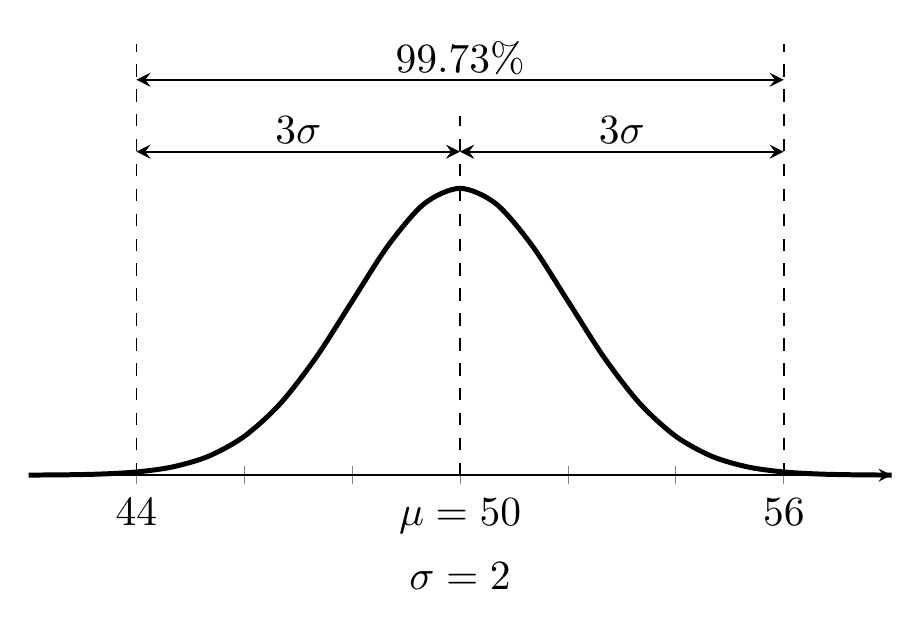
\begin{tikzpicture}[scale=1.5]
        \begin{axis}[
          domain=-4:4,
          xmin=-4, xmax=4,
          ymin=-0.3, ymax=0.7,
          width=3.5in,
          xtick={-3,-2,-1,0,1,2,3},
            xticklabels={$44$,,,$\mu=50$,,,$56$},
            axis x line=center,
            axis y line=none,
            every axis x label/.style={at=(current axis.right of origin),anchor=west},
          ]
      \addplot [very thick,  smooth] {(e^(-0.5*(x)^2))/((2*pi)^0.5)};
      \draw [dashed] (0,0) -- (0,0.5);
      \node[] at (0,-0.14)   {$\sigma=2$};
      \draw [dashed] (-3,0) -- (-3,0.6);
      \draw [dashed] (3,0) -- (3,0.6);
      \draw[line width=0.5pt, stealth-](0,0.45)--(1,0.45);
       \draw[line width=0.5pt, stealth-](3,0.45)--(1,0.45);
     \draw[line width=0.5pt, stealth-](0,0.45)--(-1,0.45);
       \draw[line width=0.5pt, stealth-](-3,0.45)--(-1,0.45);
      \node[] at (1.5,0.48)   {$3\sigma$};
      \node[] at (-1.5,0.48)   {$3\sigma$};
      \draw[line width=0.5pt, stealth-](-3,0.55)--(0,0.55);
      \draw[line width=0.5pt, stealth-](3,0.55)--(0,0.55);
      \node[] at (0,0.58)   {$99.73\%$};
      \end{axis}
        \end{tikzpicture}
\end{center}
    
        Observe that $50-3\sigma=44$ and $50+3\sigma=56$.  By the Empirical Rule, $99.73\%$ of the data lies between $44$ and $56$.  The end-points of this interval just happen to coincide with the spec limits.  In other words, the spec limits are located at $\pm 3\sigma$ away from the mean.  Therefore, $99.73\%=0.9973$ of output falls within the spec limits.  This may seem like a good thing, but if we fill an order of $1,000,000$ parts using Machine 1, then the number of defective screws will be approximately
        $$(1-0.9973)\times 1,000,000=0.0027\times 1,000,000=2,700$$       
    \end{explanation}
\end{example}

\begin{question}\label{quest:defParts1}
    Suppose that a new employee was assigned to Machine 1 and the machine's performance changed as a result.   The output of the machine can now be described using normal distribution with mean $\mu=50$ and standard deviation $\sigma=3$.  Your goal is to approximate the number of defective screws per one million.

    Recall that $LSL=44$ mm and $USL=56$ mm. Where are the spec limits in relation to the center of this distribution?

    \begin{multipleChoice}
        \choice{The spec limits are at $\pm \sigma$.}
        \choice[correct]{The spec limits are at $\pm 2\sigma$.}
        \choice{The spec limits are at $\pm 3\sigma$.}
    \end{multipleChoice}

Rounded to the nearest integer, what percent of data is located within the spec limits?

Percent of data within spec limits: $\answer{95}\%$

How many defective parts per million do we expect to see?  

Defective parts per million: $\answer{50000}$ ppm

Compare your answer to this question with Example \ref{ex:defParts1}.  Which of the following is true about a normally distributed process?

\begin{multipleChoice}
\choice{If the process mean is unchanged, then the amount of scrap remains the same regardless of what happens to standard deviation.}
    \choice[correct]{If the process mean is unchanged, then greater standard deviation leads to more scrap.}
    \choice{If the process mean is unchanged, then smaller standard deviation leads to more scrap.}
    \end{multipleChoice}
    \end{question}

Process mean and standard deviation both affect the amount of scrap produced by the process.  The Desmos interactive below allows you to visualize the number of defective parts that result from a normally distributed processes with various means and standard deviations.  Use the sliders on the left to change the mean and standard deviation of the distribution and observe how the number of defective parts changes.

\begin{onlineOnly}
\begin{center} 
\desmos{f95viwzyer}{800}{600} 
\end{center}
\end{onlineOnly}

\begin{question}\label{ex:defParts3}
    Suppose that the output of Machine 2 can be described using normal distribution with mean $\mu=50$ and standard deviation $\sigma=1$.  If a batch of $1,000,000$ is ordered, how many defective screws do you expect?  Use the Desmos interactive above to find out.  Round your answer to three decimal places.

    Number of defective parts per million: $\answer{0.002}$ ppm.

    If the mean of Machine 2 shifts to $51.3$, with $\sigma =1$, how many defective parts per million do you expect?  Round your answer to one decimal place.

    Number of defective parts per million: $\answer{1.3}$ ppm.
\end{question}

\subsection*{Process Capability and Quality Standards}
At this point you should have an idea of how the histogram needs to be positioned in relation to the spec limits in order to minimize scrap.  Let's summarize these characteristics.  
\begin{question}\label{prob:specs1}
Select a combination of TWO conditions that will result in the smallest amount of scrap.

    \begin{selectAll}
        \choice[correct]{data are centered between the spec limits}
        \choice{data are shifted to the low side}
        \choice{data are shifted to the high side}
        \choice[correct]{process width is narrower than the spec width.}
        \choice{process width is the same as spec width.}
        \choice{process width is greater than spec width.}
    \end{selectAll}
\end{question}

We will now quantify your observations in Question \ref{prob:specs1}.  The \emph{process potential} ($Cp$) and \emph{process capability} ($Cpk$) formulas below use ratios to allow us to numerically assess the width of the bell curve and its location in relation to the spec limits.  Process potential and process capability are the two primary indicators for process capability.

\begin{center}
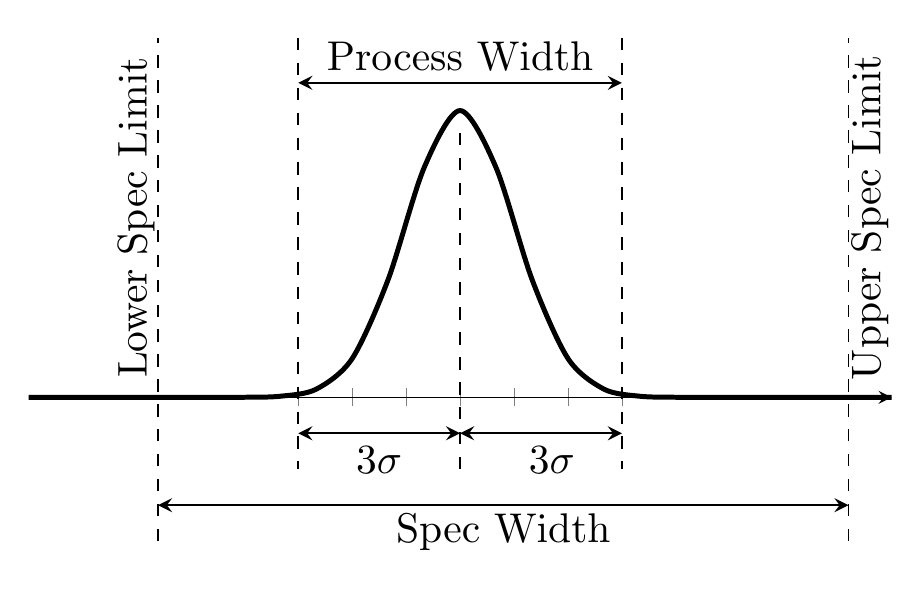
\begin{tikzpicture}[scale=1.5]
        \begin{axis}[
          domain=280:320,
          xmin=280, xmax=320,
          ymin=-0.1, ymax=0.3,
          width=3.5in,
          xtick={292.5, 295, 297.5,300,302.5,305, 307.5},
            xticklabels={,,,,,,},
           % ytick style={draw=none},
            %yticklabels={},
            axis x line=center,
            axis y line=none,
          %axis lines =middle, xlabel={}, ylabel={},
          %every axis y label/.style={at=(current axis.above origin),anchor=south},
           every axis x label/.style={at=(current axis.right of origin),anchor=west},
          ]
      \addplot [very thick,  smooth] {(e^(-0.5*((x-300)/2.5)^2))/(((2*pi)^0.5)*2.5)};
      \draw [dashed] (300,-0.04) -- (300,0.15);
      \draw [dashed] (286,-0.08) -- (286,0.2);
      \draw [dashed] (318,-0.08) -- (318,0.2);
      \draw [dashed] (292.5,0.2) -- (292.5,-0.04);
      \draw [dashed] (307.5,0.2) -- (307.5,-0.04);
      \node[rotate=90] at (285,0.1)   {Lower Spec Limit};
      \node[rotate=90] at (319,0.1)   {Upper Spec Limit};
      \draw[line width=0.5pt, stealth-](300,-0.02)--(305.5,-0.02);
      \draw[line width=0.5pt, stealth-](307.5,-0.02)--(305.5,-0.02);
      \draw[line width=0.5pt, stealth-](300,-0.02)--(295.5,-0.02);
      \draw[line width=0.5pt, -stealth](295.5,-0.02)--(292.5,-0.02);
      \node[] at (296.25,-0.035)   {$3\sigma$};
      \node[] at (304.25,-0.035)   {$3\sigma$};
      \draw[line width=0.5pt, -stealth](300,-0.06)--(318,-0.06);
      \draw[line width=0.5pt, -stealth](300,-0.06)--(286,-0.06);
       \node[] at (302,-0.075)   {Spec Width};
       \draw[line width=0.5pt, -stealth](300,0.175)--(307.5,0.175);
      %\draw[line width=0.5pt, stealth-](307.5,0.18)--(305.5,0.18);
      \draw[line width=0.5pt, -stealth](300,0.175)--(292.5,0.175);
      %\draw[line width=0.5pt, -stealth](295.5,-0.02)--(292.5,-0.02);
      \node[] at (300,0.19)   {Process Width};
          \end{axis}
        \end{tikzpicture}
\end{center}

Given the process's standard deviation, $\sigma$, we know that $99.73\%$ of the data are located within three standard deviations of the mean.  In other words, $99.73\%$ of data lie along an interval of length $6\sigma$.  This length is sometimes referred to as \emph{process width}.

\begin{formula}[Process Potential]\label{form:Cp}
$$Cp=\frac{\text{Spec Width}}{\text{Process Width}}=\frac{\text{Upper Spec Limit}-\text{Lower Spec Limit}}{6\sigma}$$
\end{formula}

Examine the fractions in the above formula to answer the following questions.  (Hint: consider what happens when the numerator is greater than the denominator and vice versa.)

 If the process width is narrower than the spec width, then $Cp$ is \wordChoice{\choice[correct]{greater than 1}, \choice{less than 1},\choice{equal to 1}}

 If the process width is wider than the spec width, then $Cp$ is \wordChoice{\choice{greater than 1}, \choice[correct]{less than 1},\choice{equal to 1}}

 If the process width is equal to the spec width, then $Cp$ is \wordChoice{\choice{greater than 1}, \choice{less than 1},\choice[correct]{equal to 1}}

 Process potential ($Cp$) tells us how process width compares to spec width, but it does not tell us where the curve is located in relation to the spec limits.  The next formula will take location into account.

\begin{formula}[Process Capability]\label{form:Cpk}
$$Cpk=\frac{\text{Distance from Mean to the nearest Spec Limit}}{3\sigma}$$
\end{formula}

Observe that both $Cp$ and $Cpk$ are unitless values.  This is because the units in the numerator and the denominator are the same and they cancel out.

$Cp$ is an internal measure for a company to track how good a process can be while $Cpk$ is the value that a company sends to their customer along with the product shipment to indicate the level of product quality. If the process is centered within the specification limits, then $Cpk$ equals $Cp$.  

The generally accepted minimum value for $Cp$ and $Cpk$ is $1.33$.  A centered process with a $Cp$ of $1.33$ results in about 66 parts per million defects.  A centered process with a $Cp$ of $1.67$ is less than one part per million defects. 

\begin{example}\label{ex:CpCpk}
    Given the following illustration of the process, find $Cp$ and $Cpk$.  What do the numbers tell us about the process?
    \begin{center}
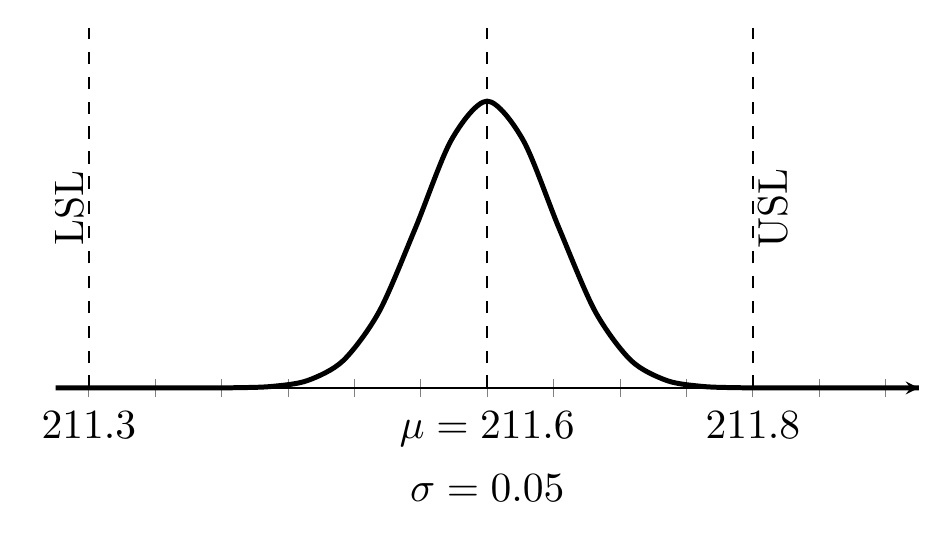
\begin{tikzpicture}[scale=1.5]
        \begin{axis}[
          domain=-6.5:6.5,
          xmin=-6.5, xmax=6.5,
          ymin=-0.3, ymax=0.7,
          width=3.5in,
          xtick={-6,-5,-4,-3,-2,-1,0,1,2,3,4,5,6},
            xticklabels={$211.3$,,,,,,$\mu=211.6$,,,,$211.8$,,},
            axis x line=center,
            axis y line=none,
            every axis x label/.style={at=(current axis.right of origin),anchor=west},
          ]
      \addplot [very thick,  smooth] {(e^(-0.5*(x)^2))/((2*pi)^0.5)};
      \draw [dashed] (0,0) -- (0,0.5);
      \draw [dashed] (-6,0) -- (-6,0.5);
      \draw [dashed] (4,0) -- (4,0.5);
      \node[rotate=90] at (-6.3,0.25)   {LSL};
      \node[rotate=90] at (4.3,0.25)   {USL};
      \node[] at (0,-0.14)   {$\sigma=0.05$};
      \end{axis}
        \end{tikzpicture}
\end{center}

\begin{explanation}
    $$Cp=\frac{211.8-211.3}{6(0.05)}=\frac{0.5}{0.3}\approx 1.67$$
This value indicates that the bell curve is narrower than the spec width.  This is good.

$$Cpk=\frac{211.8-211.6}{3(0.05)}=\frac{0.2}{0.15}\approx 1.33$$
Unlike $Cp$, $Cpk$ takes the position of the curve within the spec limits into account.  In this case $Cp\neq Cpk$ because the bell curve is not centered between the spec limits.  We use the spec limit closest to the mean to compute $Cpk$.  This value is not as good as $Cp$, but it is still greater than 1.  
\end{explanation}
\end{example}

The following interactive allows you to change the process mean and standard deviation, and see how $Cp$ and $Cpk$ are computed.
As you change the mean and standard deviation, specification limits stay fixed. This highlights the fact that there is no inherent relationship between the specs and the process.  Specification limits are dictated by real-life requirements and often cannot be altered.  Mean and standard deviation are characteristics of a particular process and its implementation.  Steps can be taken to center the mean and to reduce process width in order to reduce scrap.

\begin{onlineOnly}
\begin{center} 
\geogebra{uu7sxwfs}{900}{500} 
\end{center}
\end{onlineOnly}

Many companies strive to achieve a centered process with a $Cp$ of 2 which results in $.0018$ defective parts per million.  This level of quality control is often considered zero defects. Use the interactive above to answer the following question.

\begin{question}\label{qest:sixSigma}
    Suppose a centered process has $Cp=2$.  Where are the spec limits located in relation to the mean?
    \begin{multipleChoice}
        \choice{The spec limits are at $\pm \sigma$.}
        \choice{The spec limits are at $\pm 2\sigma$.}
        \choice{The spec limits are at $\pm 3\sigma$.}
        \choice{The spec limits are at $\pm 4\sigma$.}
        \choice{The spec limits are at $\pm 5\sigma$.}
        \choice[correct]{The spec limits are at $\pm 6\sigma$.}
    \end{multipleChoice}

An initiative to advance this level of quality was introduced by Motorala in the mid 1980s.  It became known as the \emph{six-sigma} quality standard.
  \end{question}
 

In industry, avoiding scrap is critical. A defective part (scrap) can result in product failure. Product failure, at a minimum, leads to the loss of goodwill by the consumer and, at the worst case, can result in catastrophic failure leading to death.

\subsection*{Accuracy and Precision}

In manufacturing, a \emph{precise} process is one that is experiencing small variation. An \emph{accurate} process is one that is manufacturing products to the desired or target size. A process can be precise but not accurate. For example, the process might be misadjusted and consistently making parts too small (or too large) but with little variation.  Similarly, a process might be making parts close to the desired size but is not consistent in size from part to part.  The average of dimensions is an indicator of process accuracy while standard deviation is an indicator of precision. 

The following is a visual summary of accuracy and precision.

\begin{center}
        \begin{tikzpicture}
\node[inner sep=0pt, anchor=base] (p1) at (0,0)
  {\includegraphics[height=70mm]{target.jpg}};
           \end{tikzpicture}
      \end{center}

Accuracy and precision can also be visualized using histograms, or graphs of distributions.  If the histogram is well-centered within the specification limits, then the process is \emph{accurate}. That is, the process is making product that is close to the nominal or midpoint of the specification range.

If the spread of the data is as wide as the specification limits, then the data is not very \emph{precise}, and the process is likely to be making scrap.

Use the sliders in the GeoGebra interactive below to visualize accuracy and precision.
\begin{onlineOnly}
\begin{center} 
\geogebra{xpfp98rz}{700}{600} 
\end{center}
\end{onlineOnly}

\subsection*{Summary}

In manufacturing, the length of a bolt, weight of cookies, fill level in a bottling operation, and the thickness of a metal layer resulting from a chemical vapor deposition (CVD) are examples of data collected and used to evaluate a process.  The type of measuring instrument used in these manufacturing operations varies considerably in terms of precision, units, sophistication, and more, but the purpose is the same: to assess the stability and quality of the manufacturing process and the product being manufactured. 

Data collected in the shop is usually recorded in a list format such as the data recorded from Machines 1 and 2 in the previous example (Evaluating Process Quality). It is difficult to evaluate a process from a list of data. Therefore, it is common to draw a picture of the data in the form of a histogram.

In addition to visual tools, data analysis is also done using statistics such as determining mean and standard deviation of the data or subsets of data.  These metrics are compared to product specifications to determine process capability and stability. 
Proper interpretation of the visual tools and calculated metrics requires a solid understanding of statistics and is critical to effective evaluation of a manufacturing process. 





% Histograms provide three pieces of information about the data:
% \begin{itemize}
%     \item Shape of data.  Measurements from a production process are typically normally distributed.  
%     \item Accuracy.  The histogram must be centered between the specification limits.  
%     \item Precision.  The histogram should roughly occupy the middle half of the space between the spec limits. 
% \end{itemize}
% If the histogram is not bell-shaped, well-centered within the spec limits or is too wide, the process needs to be paused and evaluated.



\section*{Practice Problems}

\begin{problem}\label{prob:lengthAreaVolume}
    For each example, select an appropriate type of measurement.

    (a)	An injection molding process produces parts with an area of 50 square millimeters: \wordChoice{\choice{Length}, \choice[correct]{Area},\choice{Volume}}

    (b) A wire that is 12 millimeters long is tested for pull strength: \wordChoice{\choice[correct]{Length}, \choice{Area},\choice{Volume}}

    (c)	Bottles are filled with 800 cubic centimeters of cleaning solution: \wordChoice{\choice{Length}, \choice{Area},\choice[correct]{Volume}}
\end{problem}

\begin{problem}\label{prob:prob2a}
A manufacturing process has the following specifications: $50$mm $\pm6$mm.
Use this list of data, rounded to the nearest half a millimeter (.5 mm), to answer the following questions. 

$$\begin{array}{|c|c|c|c|} 
 \hline 
 47 & 49 & 48 & 48.5\\ \hline 
 47 & 48.5 & 48 & 47.5\\ \hline 
 48 & 47.5 & 48 & 49.5\\ \hline 
 50 & 49.5 & 50 & 50.5\\ \hline 
 51 & 51.5 & 52 & 50\\ \hline 
 \end{array}$$

Calculate the following to TWO decimal places.
$$LSL=\answer{44}$$
$$USL=\answer{56}$$
$$\text{Process mean}=\mu=\answer{49.05}$$
$$\text{Process standard deviation}=\sigma=\answer{1.45}$$
$$\text{Process potential}=Cp=\answer[tolerance=0.015]{1.38}$$
$$\text{Process capability}=Cpk=\answer[tolerance=0.015]{1.16}$$

Enter the values of $\mu$ and $\sigma$ you found above into the interactive below, and note the number of defective parts per million (ppm).

\begin{onlineOnly}
\begin{center} 
\desmos{f95viwzyer}{800}{600} 
\end{center}
\end{onlineOnly}

Using a quality goal of no more than 66 parts per million defects, this process:

\begin{multipleChoice}
    \choice{Meets the quality goal.}
    \choice{Exceeds the quality goal.}
    \choice[correct]{Falls short of the quality goal.}
    \choice{Not enough information to answer this question.}
\end{multipleChoice}


\end{problem}

\section*{References}

CETB Scanning Electron Microscope photo credit: \textit{CETB Scanning Electron Microscope} by Teupdeg, GNU Free Documentation License.

Wafer photo credit: \textit{Processed 200 mm Si Wafer} by Goldenvu CC BY-SA 4.0.


\end{document} 